\section{Versuchsdurchführung}
\label{sec:durchfuerung}

\subsection{Einstellen der Temperaturprofile}
\subsubsection*{Vorbereitung des Thermostates und des Reaktors}
Begonnen wurde die Versuchsdurchführung durch Inbetriebnahme des Thermostats. Hierfür wurden die Gewebe-PVC-Schläuche über einen Schlauch-Gewinde-Adapter mit dem 2L-Reaktor verbunden. Das jeweils andere Ende der Schläuche war bereits mit dem Thermostat über Schlauchschellen befestigt. Für die Verbindung mit dem Thermostat war es zu beachten, dass der Schlauch mit dem heizenden Vorlaufstrom an der unteren Seite des Reaktors festgeschraubt wurde, Luftblasen im Reaktormantel zu vermeiden. Danach wurden ebenfalls über Schlauchschellen weitere PVC-Schläuche mit den Ein- und Ausgänge der Thermostatkühlung verbunden. Der eingehende Schlauch wurde auf der anderen Seite mit einem Wasseranschluss (ungeöffnet) versehen. Der ausgehende Schlauch führte in einen Ausguss. Nun konnte das Thermostat eingeschaltet werden und es meldete sich sofort eine Fehlermeldung E01, welche in diesem Fall auf einen zu niedrigen Füllstand im Behälter des Thermostates hinwies. Nach Auffüllen des Theromstatbades wurde das Gerät erneut ohne Fehlermeldung gestartet und nun war es dem Thermostat manuell eine Solltemperatur zu geben und den Prozess zu starten. Um jedoch mit Temperaturrampen arbeiten zu können, war das Herstellen einer Verbindung zu einem PC mit der \textsc{Julabo Easy Temp} Software nötig.

\anmerkung{Abbildung mit Thermostat Wasserhahn und Reaktor}
\subsubsection*{Konfigurieren des Thermostates}
Hierfür wurde der Computer und das Thermostat mittels Kabel über die verfügbaren RS-232-Schnittellen miteinander verbunden. Durch gleichzeitiges Drücken der Cursortaste \keys{\arrowkeyleft} und der Entertaste \keys{\return} gelangte man in die Konfigurationsebene des Thermostates und konnte die in Tabelle \ref{tab:thermostat_config} aufgeführten Einstellungen für die Fernsteuerung mittels Computer einstellen. Über die Tasten \keys{\arrowkeyleft} und \keys{\arrowkeyright} ließ sich nun der gewünschte Parameter auswählen und über die Tasten \keys{\arrowkeyup} und  \keys{\arrowkeydown} dessen Wert verändern. Jede Änderung musste mit der Entertaste \keys{\return} bestätigt werden. Durch erneut gleichzeitiges Drücken der Cursortaste \keys{\arrowkeyleft} und der Entertaste \keys{\return} wurde die Konfigurationsebene des Thermostats wieder verlassen. Auf dem Display der Thermostates war nun die Meldung \texttt{rOFF} zu sehen.
\subsubsection*{Konfigurieren des Computers}
Nachdem das Thermostat konfiguriert wurde, erfolgte eine weitere Konfiguration am PC mit der \textsc{Julabo Easy Temp} Software. Nach dem Starten des Programms wurde zu \menu{Geräte>Geräte konfigurieren} navigiert und es öffnete sich ein Fenster. Unter \menu{Gerät hinzufügen} können nun die Einstellungen aus Tabelle \ref{tab:thermostat_config} für den Computer konfiguriert werden.
\begin{table}[h!]
	\renewcommand*{\arraystretch}{1.2}
	\centering
	\caption{Konfigurationen \textsc{Julabo} Thermostat MW und \textsc{Easy Temp}-Software}
	\label{tab:thermostat_config}
	\begin{tabulary}{1.0\textwidth}{C|C|C}
		\hline
		\textbf{Gerät} & \textbf{Parameter} & \textbf{Wert}\\
		\hline
		\multirow{5}{*}{Thermostat} & \texttt{Atc} & \texttt{0}\\
		& \texttt{H} & \texttt{1}\\
		& \texttt{P} & \texttt{2}\\
		& \texttt{Br} & \texttt{48}\\
		& \texttt{r} & \texttt{1}\\
		\hline
		\multirow{3}{*}{Software} & \texttt{Gerät} & \texttt{TopTechMXs}\\
		& \texttt{Anschluss} & \texttt{COM 1}\\
		& \texttt{Bautenrate} & \texttt{48000 s}\\
		\hline			
	\end{tabulary}
\end{table}%
\FloatBarrier

Als dies erfolgt war, konnten alle Einstellungen übernommen werden und es öffnet sich ein Fenster wie in Abbildung \ref{fig:fenster_standby_online}. Über das Feld \texttt{Online} wurde bestätigt, dass eine Verbindung mit dem Thermostat hergestellt wurde. Über einen Klick auf das graue Feld \texttt{Standby} konnte das Thermostat nun gestartet werden und das Feld wechselte die Farbe auf grün und zeigte das Wort \texttt{Start} an. Das Thermostat regelte die Temperatur des Heizfluides (hier: Wasser) nun auf die angegebene Solltemperatur (hier: 80°C). Über einen Klick auf die Solltemperatur, ließ sich dieser Wert auch ändern.

\begin{figure}[h!]
	\centering
	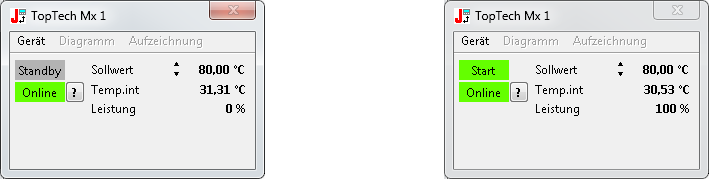
\includegraphics[width=1.0\textwidth]{img/julabo_2}
	\caption{Gerätefenster der \textsc{Easy Temp} Software zum starten des Thermostates}
	\label{fig:fenster_standby_online}
\end{figure}
\FloatBarrier
%Ende

\subsubsection*{Kurvendarstellung am PC - \textsc{Easy Temp} Software}
Nachdem nun das Thermostat und der PC miteinander kommunizieren konnten, bestand nun auch die Möglichkeit sich den Temperaturverlauf des Heißfluides darstellen zu lassen. Hierfür navigierte man im Hauptfenster des Programms nach \menu{Ansicht>Kurven bearbeiten} und es öffnete sich das Fenster der Kurvenkonfiguration, welches in Abb. \ref{fig:kurvenkonfig} zu sehen ist. Über die Schaltfläche \menu{Hinzufügen} konnte nun ein neues Gerät hinzugefügt werden, sowie der darzustellende Messwert ausgewählt und Namen für den Messwert vergeben werden. In diesem Versuch wurden der Sollwert und die interne Temperatur im Thermostat ausgewählt und infolge dieser Einstellungen geplottet (vgl. Abb. \ref{fig:beispiel_plot}).

\begin{figure}[h!]
	\centering
	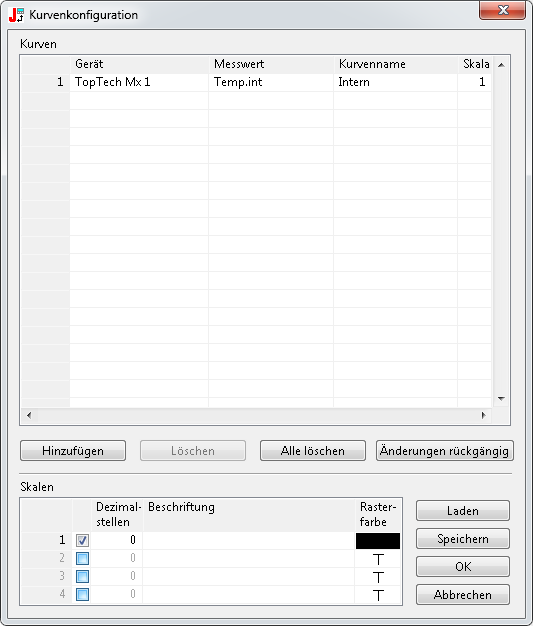
\includegraphics[width=0.5\textwidth]{img/julabo_3}
	\caption{Kurvenkonfiguration der \textsc{Easy Temp} Software}
	\label{fig:kurvenkonfig}
\end{figure}
\FloatBarrier
%Ende

\begin{figure}[h!]
	\centering
	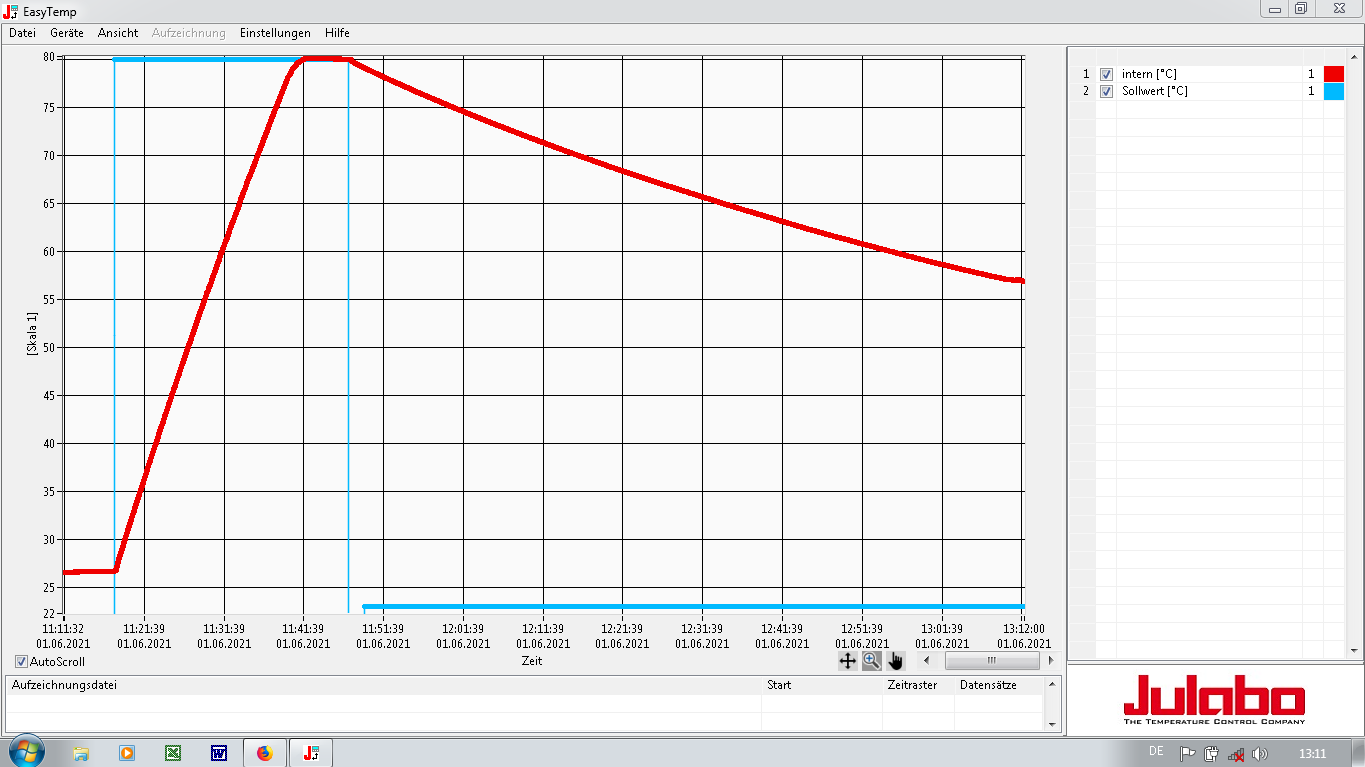
\includegraphics[width=0.75\textwidth]{img/julabo_4}
	\caption{Beispiel einer Messwertaufnahme in \textsc{Easy Temp}}
	\label{fig:beispiel_plot}
\end{figure}
\FloatBarrier
%Ende

\subsection{Messwertaufnahme der Temperaturprofile}
Da die aufgenommenen Messwerte der \textsc{Easy Temp}-Software nicht in der kostenfreien Variante des Programms exportiert werden können, war für die Messwertaufnahme eine externe Messung notwendig. Hierfür wurde das Präzisionsmessgerät \textsc{Ahlborn Almemo 2890-9} mit Thermoelementstecker genutzt. Ein Messfühler wurde dabei für die Messung der Lufttemperatur und einer für die Temperatur des Theromstatbades genutzt. Über einen passendes Datenkabel, welches in den oberen linken USB-Ports des Rechners gesteckt wurde, konnte nun über die Software \textsc{WinControl} eine exportierbare Messwertaufzeichnung realisiert werden.
Zunächst sollte überprüft werden, dass das Messgerät eine Bautenraten von \SI{9600}{\second} aufweist. Da an dem Messgerät nichts geändert wurde, konnte davon ausgegangen werden, dass diese Bautenrate bereits eingestellt ist. Es folgt das Starten des Programmes \textsc{WinControl} und über das Menü \menu{Einstellungen>Verbindungen verwalten>Hinzufügen} konnte ein Gerät hinzugefügt werden. Als Anschluss musste in diesem Versuch \texttt{COM4} gewählt werden. Eine erfolgreiche Verbindung ist am grün-blinkendem Feld am unteren Rand des Programms sichtbar (siehe Abb. \ref{fig:almemo_gerat}).

\begin{figure}[h!]
	\centering
	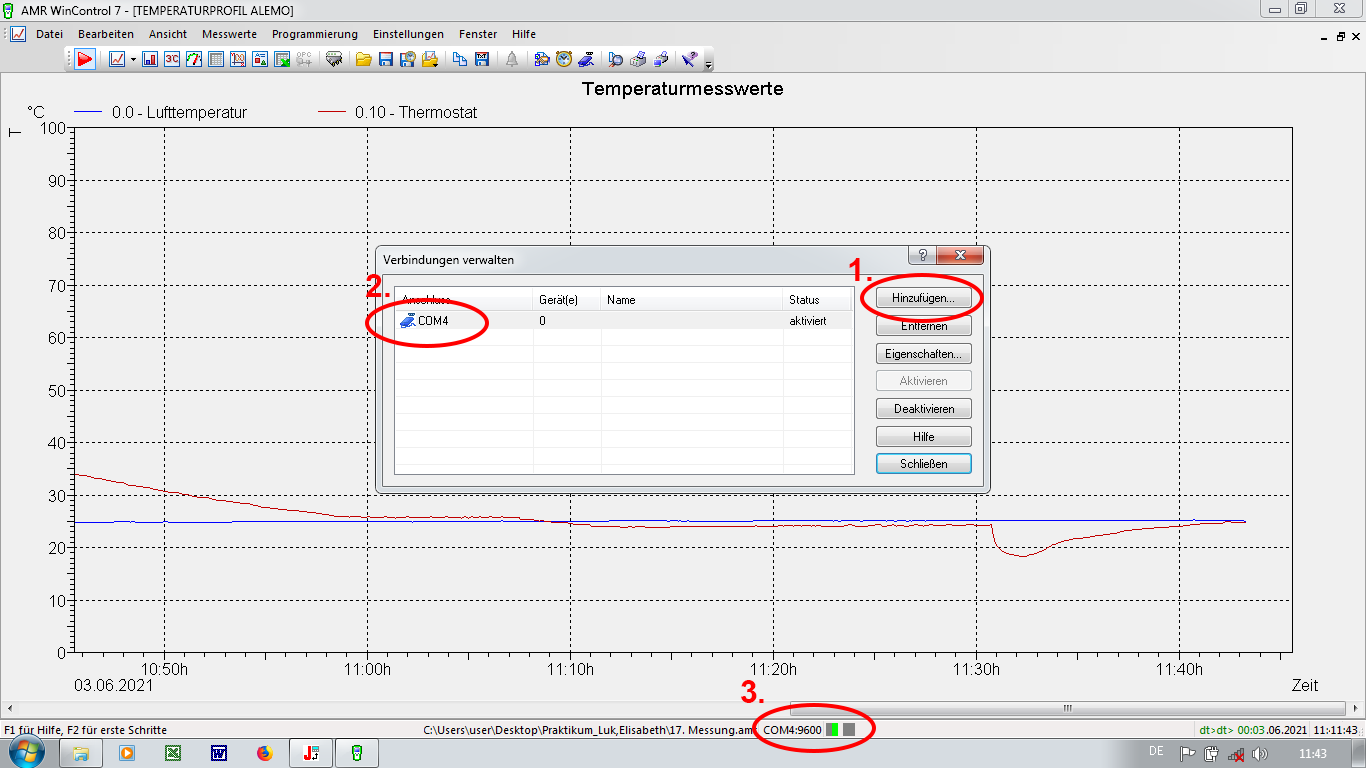
\includegraphics[width=0.75\textwidth]{img/almemo_1}
	\caption{Einrichten des Präzisionsmessgerätes mit \textsc{WinControl}}
	\label{fig:almemo_gerat}
\end{figure}
\FloatBarrier
%Ende

Nachdem das Messgerät nun von der Software erkannt wurde, konnten unter \menu{Programmierung> Messstellen programmieren>Messstellen} die Messstellen programmiert werden. Über ein Dropdown-Menü ließ sich hier die jeweilige Messstelle auswählen und über die Kommentarfunktion benennen. Als Messbereich wurde passend zum Thermoelementsstecker \texttt{NiCr} ausgewählt (siehe Abb. \ref{fig:almemo_programm}).

\begin{figure}[h!]
	\centering
	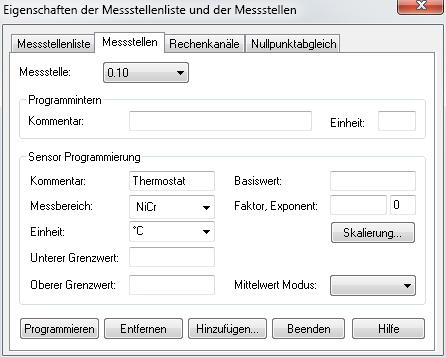
\includegraphics[width=0.5\textwidth]{img/almemo_2}
	\caption{Programmieren der Messstellen in \textsc{WinControl}}
	\label{fig:almemo_programm}
\end{figure}
\FloatBarrier
%Ende

Um im Programm nun Messwerte aufzeichnen lassen zu können muss über \menu{Messwerte>neues Liniendiagramm} ein neues Liniendiagramm eingerichtet werden. Wie in Abbildung \ref{fig:almemo_linien} zu ist, öffnete sich ein Fenster in dem sich die jeweiligen Messstellen aktivieren und dazu passende Linienfarben auswählen ließen. Unter dem Punkt \texttt{Y-Achsen} wurde zudem eine Y-Achse mit $T$ für Temperatur bezeichnet und das \texttt{Gitter} aktiviert. Danach konnten diese Einstellungen übernommen werden und die Messwertaufnahme mit der Taste \keys{F12} oder dem roten Dreieck gestartet werden.
\begin{figure}[h!]
	\centering
	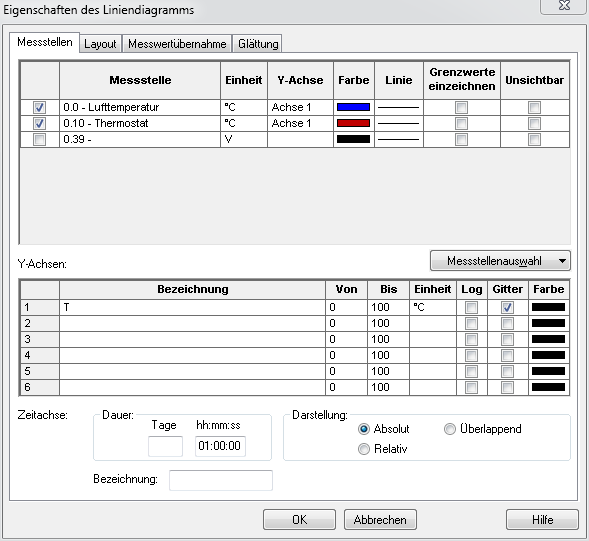
\includegraphics[width=0.5\textwidth]{img/almemo_3}
	\caption{Einrichten des Liniendiagramms in \textsc{WinControl}}
	\label{fig:almemo_linien}
\end{figure}
\FloatBarrier
%Ende
Eine mögliche Messwertaufzeichnung ist in Abb. \ref{fig:almemo_beispiel} dargestellt.
\begin{figure}[h!]
	\centering
	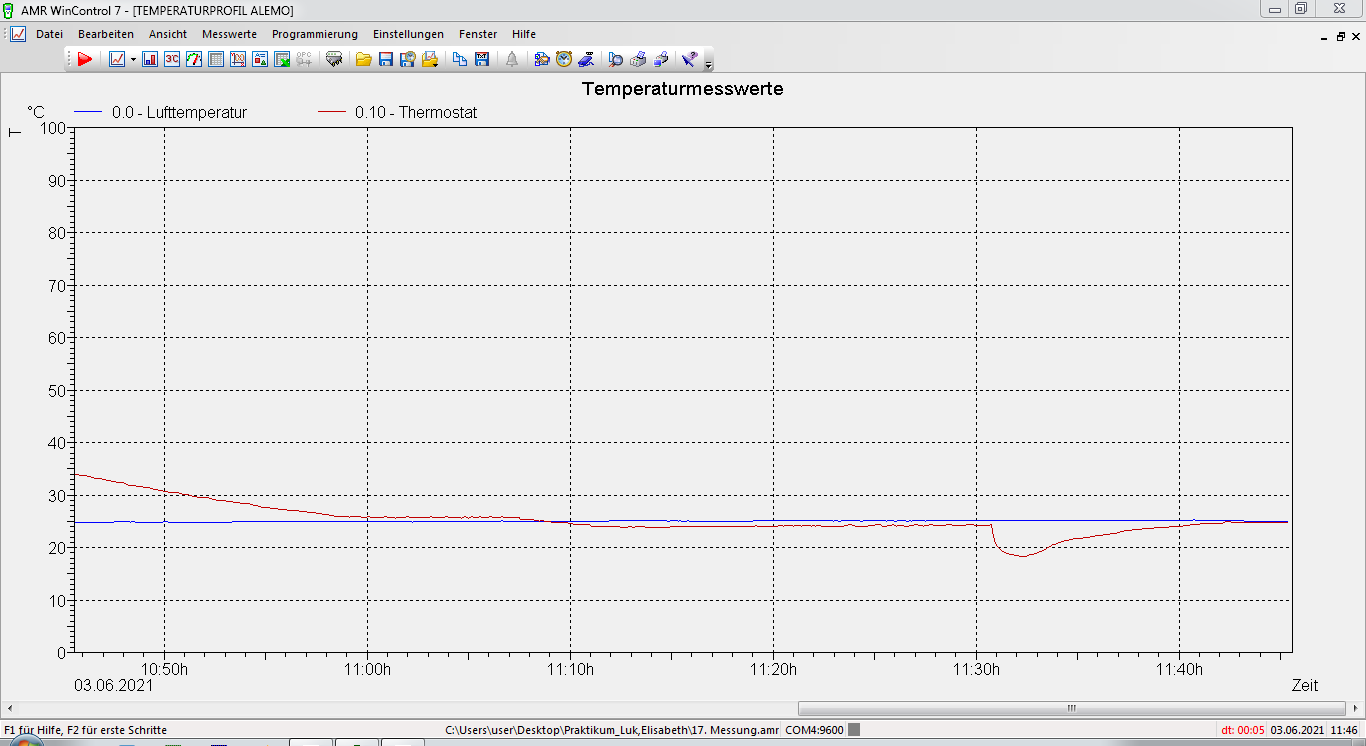
\includegraphics[width=0.5\textwidth]{img/almemo_4}
	\caption{Beispiel einer Messwertaufnahme in \textsc{WinControl}}
	\label{fig:almemo_beispiel}
\end{figure}
\FloatBarrier
%Ende
Um Messwerte mit \textsc{WinControl} wurde unter \menu{Datei>Exportieren>Excel} navigiert, alle Messstellen markiert und über die Schaltfläche \menu{senden} gespeichert.

\subsubsection*{Zeitmessung der Heiz- und Abkühlvorgänge}
Für eine grobe Abschätzung der Dauer der geforderten Prozesse wurden das Aufheizen des leeren Reaktors beginnend bei \SI{25}{\celsius} und das Abkühlen von zuvor einzustellenden \SI{80}{\celsius} wieder auf \SI{25}{\celsius} gemessen. Die \SI{25}{\celsius} werden hierbei als Raumtemperatur angenommen. Diese Abschätzungen sollten in der weiteren Versuchsdurchführung dazu dienen, die Temperaturprofile einstellen zu können.\\
Es erfolgte lediglich eine Messung bei das Thermostat mit einer Solltemperatur gestartet wurde und die Zeitmessung ab einer Temperatur von \SI{25}{\celsius} bis zum Erreichen der \SI{80}{\celsius} erfolgte. Nachdem die Solltemperatur erreicht wurde, ist diese für eine zeit von mehr als \SI{5}{\minute} gehalten worden. Danach wurde die Solltemperatur auf \SI{25}{\celsius} eingestellt und es begann die zweite Zeitmessung zusammen mit einem Kühlstrom. Hierzu wurde ein Leitungswassersstrom (\SI{23}{\celsius}, \SI{55}{\liter\per \hour}) in das Thermostat eingeleitet, um eine möglichst schnellere Kühlung zu erreichen. Für die Messung des maximalen Leitungswasserstromes wurden über drei Messreihen eine Zeit gestoppt und das aufgefangene Wasser ausgewogen.
In Tabelle \ref{tab:zeiten} sind die gemessenen Zeiten und Aufheizen und Abkühlen aufgeführt und in Tabelle \ref{tab:volumenstrom_kuehlung} sind die Messwerte für die Bestimmung des maximalen Volumenstroms des Kühlwassers aufgeführt. In Abb. \ref{dia:temp_graphen} sind alle Vorgänge nochmal für den gesamten Prozess 1 ohne Wasserdampfdestillation in einem Diagramm dargestellt.

\begin{table}[h!]
	\renewcommand*{\arraystretch}{1.2}
	\centering
	\caption{Gemessene Dauer für Aufheiz- und Abkühlvorgänge mit $\delta_{\text{Start}}=\SI{25}{\celsius}$}
	\label{tab:zeiten}
	\begin{tabulary}{1.1\textwidth}{C|C|C}
		\hline
		\textbf{Starttemperatur}&\textbf{Aufheizzeit bis $\delta=\SI{80}{\celsius}$} & \textbf{Abkühlzeit von $\delta=\SI{80}{\celsius}\rightarrow\SI{25}{\celsius}$}\\
		\SI{25}{\celsius} & \SI{24}{\minute} & \SI{24}{\minute}\\
		\hline			
	\end{tabulary}
\end{table}%
\FloatBarrier

\begin{table}[h!]
	\renewcommand*{\arraystretch}{1.2}
	\centering
	\caption{Messungen für die Bestimmung des Leitungswasserstromes ($\delta_{\text{Kühlwasser}}=\SI{23,2}{\celsius}$)}
	\label{tab:volumenstrom_kuehlung}
	\begin{tabulary}{1.1\textwidth}{C|C|C|C|C}
		\hline
		\textbf{Messreihe}& \textbf{Zeit $t \, \left[\si{\second}\right]$} & \textbf{Masse $g \, \left[\si{\gram}\right]$} & \textbf{Volumen $V \, \left[\si{\milli \liter}\right]$} & \textbf{Volumenstrom $\dot{V}\, \left[\si{\liter \per \hour}\right]$} \\
		\hline
		1 & 6,5				& 103 & 103,3 & 57,2\\
		2 & 10,0			& 146 & 146,4 & 52,7\\
		3 & 8,0				& 124 & 124,3 & 55,9\\
		\hline
		Mittelwert 	& 8,2	& 124 & 124,6 & 55,3\\ 		
		\hline	
	\end{tabulary}
\end{table}%
\FloatBarrier

\begin{figure}[h!]
	\begin{center}
		\resizebox{0.8\textwidth}{!}{
			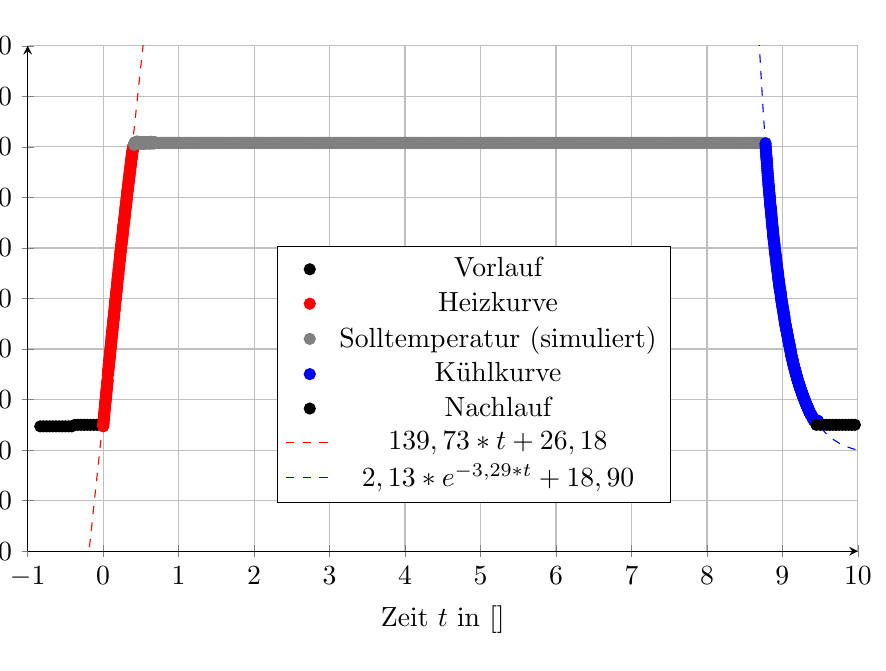
\begin{tikzpicture}[trim axis left, trim axis right]
				\begin{axis}[
					grid = major,
					axis lines = left,
					width = \textwidth,
					height = 8cm,
					xticklabel style={
						/pgf/number format/fixed,
						/pgf/number format/precision=2
					},
					xmin = -1,
					xmax = 10,
					ymin = 0,
					ymax = 100,
					ytick = {0,10,...,100},
					xtick = {-1,...,10},
					ylabel={Temperatur $\delta$ in $\left[\si{\celsius}\right]$},
					%y label style={at={(0,0.5)}},
					xlabel={Zeit $t$ in $\left[\si{\hour}\right]$},
					legend style={at={(0.3,0.35)},anchor=west},
					%	y dir = reverse,
					]
					\addplot [color=black, mark=*, only marks] coordinates{(-0.833333333333333,24.7) (-0.791666666666667,24.7) (-0.75,24.7) (-0.708333333333333,24.7) (-0.666666666666667,24.7) (-0.625,24.7) (-0.583333333333333,24.7) (-0.541666666666667,24.7) (-0.5,24.7) (-0.458333333333333,24.7) (-0.416666666666667,24.7) (-0.375,25) (-0.333333333333333,25) (-0.291666666666667,25) (-0.25,25) (-0.208333333333333,25) (-0.166666666666667,25) (-0.125,25) (-8.33333333333333E-02,25) (-4.16666666666667E-02,25) (0,25) };
					
					\addplot [color=red, mark=*, only marks] coordinates{(0,24.7) (1.38888886431239E-03,24.9) (2.7777779032477E-03,25.2) (4.16666676756002E-03,25.3) (5.55555563187234E-03,25.6) (6.94444449618466E-03,25.9) (8.33333336049698E-03,26.1) (9.7222222248093E-03,26.3) (1.11111110891216E-02,26.6) (1.24999999534339E-02,26.8) (1.38888889923692E-02,27) (1.52777778566816E-02,27.2) (1.66666667209939E-02,27.5) (1.80555555853062E-02,27.6) (1.94444444496185E-02,27.9) (2.08333333139309E-02,28.1) (2.22222221782432E-02,28.3) (2.36111112171785E-02,28.5) (2.50000000814908E-02,28.7) (2.63888889458031E-02,29) (2.77777778101154E-02,29.2) (2.91666666744278E-02,29.4) (3.05555555387401E-02,29.6) (3.19444444030524E-02,29.8) (3.33333334419877E-02,30) (0.0347222223063,30.2) (3.61111111706124E-02,30.5) (3.75000000349247E-02,30.7) (0.038888888899237,30.9) (4.02777777635493E-02,31.1) (4.16666666278616E-02,31.3) (4.30555556667969E-02,31.5) (4.44444445311093E-02,31.7) (4.58333333954216E-02,31.9) (4.72222222597339E-02,32.1) (4.86111111240462E-02,32.3) (4.99999999883585E-02,32.5) (5.13888888526709E-02,32.7) (5.27777778916062E-02,32.9) (5.41666667559185E-02,33.1) (5.53888888557753E-02,33.4) (5.67777778947106E-02,33.6) (5.81666667590229E-02,33.7) (5.95555556233352E-02,34) (6.31666667054718E-02,34.8) (6.45555555697842E-02,35) (6.59444444340965E-02,35.3) (6.73333332984088E-02,35.6) (6.87222223373441E-02,35.8) (7.01111112016564E-02,36) (7.15000000659687E-02,36.2) (7.28888889302811E-02,36.4) (7.42777777945934E-02,36.6) (7.56666666589057E-02,36.9) (0.077055555523218,37) (7.84444445621533E-02,37.2) (7.98333334264656E-02,37.4) (0.081222222290778,37.6) (8.26111111550903E-02,37.8) (8.40000000194026E-02,38) (8.53888888837149E-02,38.2) (8.67777777480273E-02,38.4) (8.81666667869626E-02,38.6) (8.95555556512749E-02,38.8) (9.09444445155872E-02,39.1) (9.23333333798995E-02,39.2) (9.37222222442118E-02,39.4) (9.51111111085242E-02,39.7) (9.64999999728365E-02,39.9) (9.78888890117718E-02,40.1) (9.92777778760841E-02,40.3) (0.100666666740396,40.5) (0.102055555604709,40.7) (0.103444444469021,40.9) (0.104833333333333,41.1) (0.106222222197646,41.3) (0.107611111236581,41.5) (0.109000000100893,41.7) (0.110388888965206,42) (0.111777777829518,42.2) (0.11316666669383,42.4) (0.114555555558143,42.6) (0.115944444422455,42.8) (0.117333333286767,42.9) (0.118722222325703,43.1) (0.120111111190015,43.3) (0.121500000054327,43.6) (0.12288888891864,43.8) (0.124277777782952,43.9) (0.125666666647264,44.2) (0.127055555511576,44.3) (0.128444444550512,44.5) (0.129833333414824,44.7) (0.131222222279136,44.9) (0.132611111143449,45) (0.134000000007761,45.4) (0.135388888872073,45.5) (0.136777777736386,45.7) (0.138166666775321,45.9) (0.139555555639633,46.1) (0.140944444503946,46.3) (0.142333333368258,46.5) (0.14372222223257,46.7) (0.145111111096883,46.9) (0.146499999961195,47.1) (0.14788888900013,47.4) (0.149277777864443,47.6) (0.150666666728755,47.7) (0.152055555593067,47.9) (0.15344444445738,48.2) (0.154833333321692,48.4) (0.156222222186004,48.6) (0.157611111224939,48.8) (0.159000000089252,49.1) (0.160388888953564,49.3) (0.161777777817876,49.5) (0.163166666682189,49.6) (0.164555555546501,49.8) (0.165944444410813,49.9) (0.167333333449749,50.1) (0.168722222314061,50.3) (0.170111111178373,50.6) (0.171500000042686,50.8) (0.172888888906998,51.1) (0.17427777777131,51.2) (0.175666666635623,51.3) (0.177055555674558,51.5) (0.17844444453887,51.8) (0.179833333403183,51.9) (0.181222222267495,52.1) (0.182611111131807,52.3) (0.18399999999612,52.5) (0.185388888860432,52.6) (0.186777777899367,53) (0.188166666763679,53.2) (0.189555555627992,53.4) (0.190944444492304,53.7) (0.192333333356616,53.9) (0.193722222220929,54) (0.195111111085241,54.2) (0.196500000124176,54.4) (0.197888888988489,54.5) (0.199277777852801,54.7) (0.200666666717113,54.9) (0.202055555581426,55) (0.203444444445738,55.3) (0.20483333331005,55.6) (0.206222222348986,55.8) (0.207611111213298,56) (0.20900000007761,56.1) (0.210388888941923,56.2) (0.211777777806235,56.4) (0.213166666670547,56.6) (0.21455555553486,56.8) (0.215944444399172,57.1) (0.217333333438107,57.4) (0.21872222230242,57.5) (0.220111111166732,57.7) (0.221500000031044,57.9) (0.222888888895356,58.2) (0.224277777759669,58.3) (0.225666666623981,58.4) (0.227055555662916,58.6) (0.228444444527229,58.9) (0.229833333391541,59.1) (0.231222222255853,59.3) (0.232611111120166,59.5) (0.233999999984478,59.6) (0.23538888884879,59.8) (0.236777777887726,60) (0.238166666752038,60.2) (0.23955555561635,60.4) (0.240944444480663,60.6) (0.242333333344975,60.7) (0.243722222209287,60.9) (0.2451111110736,61.1) (0.246500000112535,61.3) (0.247888888976847,61.6) (0.24927777784116,61.7) (0.250666666705472,61.8) (0.252055555569784,62) (0.253444444434096,62.1) (0.254833333298409,62.3) (0.256222222337344,62.5) (0.257611111201656,62.6) (0.259000000065969,62.9) (0.260388888930281,63.1) (0.261777777794593,63.4) (0.263166666658906,63.6) (0.264555555523218,63.7) (0.265944444562153,64) (0.267333333426466,64.1) (0.268722222290778,64.3) (0.27011111115509,64.5) (0.271500000019403,64.6) (0.272888888883715,64.7) (0.274277777748027,64.9) (0.275666666786963,65) (0.277055555651275,65.3) (0.278444444515587,65.5) (0.2798333333799,65.6) (0.281222222244212,65.8) (0.282611111108524,65.9) (0.283999999972836,66.1) (0.285388889011772,66.3) (0.286777777876084,66.5) (0.288166666740396,66.7) (0.289555555604709,66.9) (0.290944444469021,67.1) (0.292333333333333,67.3) (0.293722222197646,67.5) (0.295111111236581,67.7) (0.296500000100893,67.9) (0.297888888965206,68.1) (0.299277777829518,68.2) (0.30066666669383,68.3) (0.302055555558143,68.4) (0.303444444422455,68.6) (0.304833333286767,68.8) (0.306222222325703,69) (0.307611111190015,69.2) (0.309000000054327,69.4) (0.31038888891864,69.6) (0.311777777782952,69.8) (0.313166666647264,70) (0.314555555511576,70.2) (0.315944444550512,70.4) (0.317333333414824,70.5) (0.318722222279136,70.7) (0.320111111143449,71) (0.321500000007761,71.1) (0.322888888872073,71.3) (0.324277777736386,71.4) (0.325666666775321,71.6) (0.327055555639633,71.7) (0.328444444503946,71.8) (0.329833333368258,72.1) (0.33122222223257,72.2) (0.332611111096883,72.4) (0.333999999961195,72.6) (0.33538888900013,72.8) (0.336777777864443,73) (0.338166666728755,73.2) (0.339555555593067,73.3) (0.34094444445738,73.6) (0.342333333321692,73.7) (0.343722222186004,73.9) (0.345111111224939,74) (0.346500000089252,74.3) (0.347888888953564,74.2) (0.349277777817876,74.5) (0.350666666682189,74.8) (0.352055555546501,74.8) (0.353444444410813,75.1) (0.354833333449749,75.2) (0.356222222314061,75.3) (0.357611111178373,75.6) (0.359000000042686,75.6) (0.360388888906998,76) (0.36177777777131,76) (0.363166666635623,76.2) (0.364555555674558,76.4) (0.36594444453887,76.5) (0.367333333403183,76.8) (0.368722222267495,76.9) (0.370111111131807,77.1) (0.37149999999612,77.2) (0.372888888860432,77.5) (0.374277777899367,77.6) (0.375666666763679,77.6) (0.377055555627992,78) (0.378444444492304,78) (0.379833333356616,78.2) (0.381222222220929,78.5) (0.382611111085241,78.5) (0.384000000124176,78.6) (0.385388888988489,78.9) (0.386777777852801,79) (0.388166666717113,79) (0.389555555581426,79.2) (0.390944444445738,79.4) (0.39233333331005,79.4) (0.393722222348986,79.6) (0.395111111213298,79.7) (0.39650000007761,79.7) (0.397888888941923,79.8) (0.399277777806235,80.1) (0.400666666670547,80) (0.40205555553486,80.1) (0.403444444399172,80.3) (0.404833333438107,80.3) (0.40622222230242,80.2) (0.407611111166732,80.4) (0.409000000031044,80.5)  };
					
					\addplot [color=gray, mark=*, only marks] coordinates{(0.410388888895356,80.4) (0.411777777759669,80.6) (0.413166666623981,80.7) (0.414555555662916,80.6) (0.415944444527229,80.8) (0.417333333391541,80.7) (0.418722222255853,80.7) (0.420111111120166,80.8) (0.421499999984478,80.8) (0.42288888884879,80.8) (0.424277777887726,80.9) (0.425666666752038,80.9) (0.42705555561635,80.8) (0.428444444480663,80.9) (0.429833333344975,80.9) (0.431222222209287,80.8) (0.4326111110736,80.9) (0.434000000112535,80.9) (0.435388888976847,80.9) (0.43677777784116,80.8) (0.438166666705472,80.8) (0.439555555569784,81) (0.440944444434096,81) (0.442333333298409,80.9) (0.443722222337344,80.8) (0.445111111201656,80.9) (0.446500000065969,81) (0.447888888930281,80.8) (0.449277777794593,80.8) (0.450666666658906,81) (0.452055555523218,80.9) (0.453444444562153,80.8) (0.454833333426466,80.9) (0.456222222290778,80.9) (0.45761111115509,80.8) (0.459000000019403,80.8) (0.460388888883715,80.9) (0.461777777748027,80.8) (0.463166666786963,80.8) (0.464555555651275,81) (0.465944444515587,80.9) (0.4673333333799,80.7) (0.468722222244212,80.8) (0.470111111108524,80.9) (0.471499999972836,80.8) (0.472888889011772,80.8) (0.474277777876084,80.8) (0.475666666740396,80.9) (0.477055555604709,80.8) (0.478444444469021,80.8) (0.479833333333333,80.7) (0.481222222197646,80.8) (0.482611111236581,80.9) (0.484000000100893,80.8) (0.485388888965206,80.7) (0.486777777829518,80.8) (0.48816666669383,80.8) (0.489555555558143,80.9) (0.490944444422455,80.8) (0.492333333286767,80.8) (0.493722222325703,80.8) (0.495111111190015,80.7) (0.496500000054327,80.7) (0.49788888891864,80.7) (0.499277777782952,80.7) (0.500666666647264,80.8) (0.502055555511576,80.9) (0.503444444550512,80.8) (0.504833333414824,80.8) (0.506222222279136,80.7) (0.507611111143449,80.6) (0.509000000007761,80.7) (0.510388888872073,80.7) (0.511777777736386,80.8) (0.513166666775321,80.8) (0.514555555639633,80.8) (0.515944444503946,80.8) (0.517333333368258,80.7) (0.51872222223257,80.7) (0.520111111096883,80.7) (0.521499999961195,80.8) (0.52288888900013,80.9) (0.524277777864443,80.8) (0.525666666728755,80.8) (0.527055555593067,80.7) (0.528444444457379,80.7) (0.529833333321692,80.7) (0.531222222186004,80.8) (0.532611111224939,80.9) (0.534000000089252,80.8) (0.535388888953564,80.8) (0.536777777817877,80.7) (0.538166666682189,80.7) (0.539555555546501,80.7) (0.540944444410813,80.7) (0.542333333449749,80.9) (0.543722222314061,80.9) (0.545111111178373,80.8) (0.546500000042686,80.8) (0.547888888906998,80.8) (0.54927777777131,80.7) (0.550666666635623,80.7) (0.552055555674558,80.8) (0.55344444453887,80.8) (0.554833333403183,80.8) (0.556222222267495,80.9) (0.557611111131807,80.9) (0.55899999999612,80.8) (0.560388888860432,80.8) (0.561777777899367,80.8) (0.56316666676368,80.7) (0.564555555627992,80.7) (0.565944444492304,80.8) (0.567333333356617,80.8) (0.568722222220929,80.8) (0.570111111085241,80.9) (0.571500000124176,80.9) (0.572888888988489,80.8) (0.574277777852801,80.8) (0.575666666717113,80.8) (0.577055555581426,80.7) (0.578444444445738,80.7) (0.57983333331005,80.8) (0.581222222348986,80.8) (0.582611111213298,80.9) (0.58400000007761,80.9) (0.585388888941923,80.9) (0.586777777806235,80.9) (0.588166666670547,80.9) (0.58955555553486,80.9) (0.590944444399172,80.9) (0.592333333438107,80.9) (0.59372222230242,80.8) (0.595111111166732,80.8) (0.596500000031044,80.8) (0.597888888895357,80.7) (0.599277777759669,80.8) (0.600666666623981,80.8) (0.602055555662916,80.9) (0.603444444527229,80.9) (0.604833333391541,80.8) (0.606222222255853,80.8) (0.607611111120166,80.7) (0.608999999984478,80.7) (0.61038888884879,80.8) (0.611777777887726,80.8) (0.613166666752038,80.9) (0.61455555561635,80.8) (0.615944444480663,80.8) (0.617333333344975,80.7) (0.618722222209287,80.8) (0.6201111110736,80.8) (0.621500000112535,80.9) (0.622888888976847,80.8) (0.62427777784116,80.7) (0.625666666705472,80.7) (0.627055555569784,80.8) (0.628444444434097,81) (0.629833333298409,80.9) (0.631222222337344,80.8) (0.632611111201656,80.7) (0.634000000065969,80.8) (0.635388888930281,80.8) (0.636777777794593,81) (0.638166666658906,80.9) (0.639555555523218,80.9) (0.640944444562153,80.8) (0.642333333426466,80.8) (0.643722222290778,80.8) (0.64511111115509,80.8) (0.646500000019403,80.9) (0.647888888883715,80.9) (0.649277777748027,80.8) (0.650666666786963,80.7) (0.652055555651275,80.8) (0.653444444515587,80.8) (0.6548333333799,80.8) (0.656222222244212,80.9) (0.657611111108524,80.9) (0.658999999972837,80.9) (0.660388889011772,80.8) (0.661777777876084,80.7) (0.663166666740396,80.8) (0.664555555604709,80.9) (0.665944444469021,80.9) (0.667333333333333,80.9) (0.668722222197646,80.8) (0.670111111236581,80.7) (0.671500000100893,80.8) (0.672888888965206,80.8) (0.674277777829518,80.8) (0.67566666669383,80.9) (0.677055555558143,80.9) (0.678444444422455,80.9) (0.679833333286767,80.8) (0.681222222325703,80.7) (0.682611111190015,80.8) (0.684000000054327,80.8) (0.68538888891864,80.8) (0.686777777782952,80.8) (0.688166666647264,80.8) (0.689555555511577,80.8) (0.690944444550512,80.9) (0.692333333414824,80.7877358490564) (0.709000000081491,80.7877358490564) (0.725666666748157,80.7877358490564) (0.742333333414824,80.7877358490564) (0.759000000081491,80.7877358490564) (0.775666666748158,80.7877358490564) (0.792333333414824,80.7877358490564) (0.809000000081491,80.7877358490564) (0.825666666748157,80.7877358490564) (0.842333333414824,80.7877358490564) (0.859000000081491,80.7877358490564) (0.875666666748158,80.7877358490564) (0.892333333414824,80.7877358490564) (0.909000000081491,80.7877358490564) (0.925666666748157,80.7877358490564) (0.942333333414824,80.7877358490564) (0.959000000081491,80.7877358490564) (0.975666666748157,80.7877358490564) (0.992333333414824,80.7877358490564) (1.00900000008149,80.7877358490564) (1.02566666674816,80.7877358490564) (1.04233333341482,80.7877358490564) (1.05900000008149,80.7877358490564) (1.07566666674816,80.7877358490564) (1.09233333341482,80.7877358490564) (1.10900000008149,80.7877358490564) (1.12566666674816,80.7877358490564) (1.14233333341482,80.7877358490564) (1.15900000008149,80.7877358490564) (1.17566666674816,80.7877358490564) (1.19233333341482,80.7877358490564) (1.20900000008149,80.7877358490564) (1.22566666674816,80.7877358490564) (1.24233333341482,80.7877358490564) (1.25900000008149,80.7877358490564) (1.27566666674816,80.7877358490564) (1.29233333341482,80.7877358490564) (1.30900000008149,80.7877358490564) (1.32566666674816,80.7877358490564) (1.34233333341482,80.7877358490564) (1.35900000008149,80.7877358490564) (1.37566666674816,80.7877358490564) (1.39233333341482,80.7877358490564) (1.40900000008149,80.7877358490564) (1.42566666674816,80.7877358490564) (1.44233333341482,80.7877358490564) (1.45900000008149,80.7877358490564) (1.47566666674816,80.7877358490564) (1.49233333341482,80.7877358490564) (1.50900000008149,80.7877358490564) (1.52566666674816,80.7877358490564) (1.54233333341482,80.7877358490564) (1.55900000008149,80.7877358490564) (1.57566666674816,80.7877358490564) (1.59233333341482,80.7877358490564) (1.60900000008149,80.7877358490564) (1.62566666674816,80.7877358490564) (1.64233333341482,80.7877358490564) (1.65900000008149,80.7877358490564) (1.67566666674816,80.7877358490564) (1.69233333341482,80.7877358490564) (1.70900000008149,80.7877358490564) (1.72566666674816,80.7877358490564) (1.74233333341482,80.7877358490564) (1.75900000008149,80.7877358490564) (1.77566666674816,80.7877358490564) (1.79233333341482,80.7877358490564) (1.80900000008149,80.7877358490564) (1.82566666674816,80.7877358490564) (1.84233333341482,80.7877358490564) (1.85900000008149,80.7877358490564) (1.87566666674816,80.7877358490564) (1.89233333341482,80.7877358490564) (1.90900000008149,80.7877358490564) (1.92566666674816,80.7877358490564) (1.94233333341482,80.7877358490564) (1.95900000008149,80.7877358490564) (1.97566666674816,80.7877358490564) (1.99233333341482,80.7877358490564) (2.00900000008149,80.7877358490564) (2.02566666674816,80.7877358490564) (2.04233333341482,80.7877358490564) (2.05900000008149,80.7877358490564) (2.07566666674816,80.7877358490564) (2.09233333341482,80.7877358490564) (2.10900000008149,80.7877358490564) (2.12566666674816,80.7877358490564) (2.14233333341482,80.7877358490564) (2.15900000008149,80.7877358490564) (2.17566666674816,80.7877358490564) (2.19233333341482,80.7877358490564) (2.20900000008149,80.7877358490564) (2.22566666674816,80.7877358490564) (2.24233333341482,80.7877358490564) (2.25900000008149,80.7877358490564) (2.27566666674816,80.7877358490564) (2.29233333341482,80.7877358490564) (2.30900000008149,80.7877358490564) (2.32566666674816,80.7877358490564) (2.34233333341482,80.7877358490564) (2.35900000008149,80.7877358490564) (2.37566666674816,80.7877358490564) (2.39233333341482,80.7877358490564) (2.40900000008149,80.7877358490564) (2.42566666674816,80.7877358490564) (2.44233333341482,80.7877358490564) (2.45900000008149,80.7877358490564) (2.47566666674816,80.7877358490564) (2.49233333341482,80.7877358490564) (2.50900000008149,80.7877358490564) (2.52566666674816,80.7877358490564) (2.54233333341482,80.7877358490564) (2.55900000008149,80.7877358490564) (2.57566666674816,80.7877358490564) (2.59233333341482,80.7877358490564) (2.60900000008149,80.7877358490564) (2.62566666674816,80.7877358490564) (2.64233333341482,80.7877358490564) (2.65900000008149,80.7877358490564) (2.67566666674816,80.7877358490564) (2.69233333341482,80.7877358490564) (2.70900000008149,80.7877358490564) (2.72566666674816,80.7877358490564) (2.74233333341482,80.7877358490564) (2.75900000008149,80.7877358490564) (2.77566666674816,80.7877358490564) (2.79233333341482,80.7877358490564) (2.80900000008149,80.7877358490564) (2.82566666674816,80.7877358490564) (2.84233333341482,80.7877358490564) (2.85900000008149,80.7877358490564) (2.87566666674816,80.7877358490564) (2.89233333341482,80.7877358490564) (2.90900000008149,80.7877358490564) (2.92566666674816,80.7877358490564) (2.94233333341482,80.7877358490564) (2.95900000008149,80.7877358490564) (2.97566666674816,80.7877358490564) (2.99233333341482,80.7877358490564) (3.00900000008149,80.7877358490564) (3.02566666674816,80.7877358490564) (3.04233333341482,80.7877358490564) (3.05900000008149,80.7877358490564) (3.07566666674816,80.7877358490564) (3.09233333341482,80.7877358490564) (3.10900000008149,80.7877358490564) (3.12566666674816,80.7877358490564) (3.14233333341482,80.7877358490564) (3.15900000008149,80.7877358490564) (3.17566666674816,80.7877358490564) (3.19233333341482,80.7877358490564) (3.20900000008149,80.7877358490564) (3.22566666674816,80.7877358490564) (3.24233333341482,80.7877358490564) (3.25900000008149,80.7877358490564) (3.27566666674816,80.7877358490564) (3.29233333341482,80.7877358490564) (3.30900000008149,80.7877358490564) (3.32566666674816,80.7877358490564) (3.34233333341482,80.7877358490564) (3.35900000008149,80.7877358490564) (3.37566666674816,80.7877358490564) (3.39233333341482,80.7877358490564) (3.40900000008149,80.7877358490564) (3.42566666674816,80.7877358490564) (3.44233333341482,80.7877358490564) (3.45900000008149,80.7877358490564) (3.47566666674816,80.7877358490564) (3.49233333341482,80.7877358490564) (3.50900000008149,80.7877358490564) (3.52566666674816,80.7877358490564) (3.54233333341482,80.7877358490564) (3.55900000008149,80.7877358490564) (3.57566666674816,80.7877358490564) (3.59233333341482,80.7877358490564) (3.60900000008149,80.7877358490564) (3.62566666674816,80.7877358490564) (3.64233333341482,80.7877358490564) (3.65900000008149,80.7877358490564) (3.67566666674816,80.7877358490564) (3.69233333341482,80.7877358490564) (3.70900000008149,80.7877358490564) (3.72566666674816,80.7877358490564) (3.74233333341482,80.7877358490564) (3.75900000008149,80.7877358490564) (3.77566666674816,80.7877358490564) (3.79233333341482,80.7877358490564) (3.80900000008149,80.7877358490564) (3.82566666674816,80.7877358490564) (3.84233333341482,80.7877358490564) (3.85900000008149,80.7877358490564) (3.87566666674816,80.7877358490564) (3.89233333341482,80.7877358490564) (3.90900000008149,80.7877358490564) (3.92566666674816,80.7877358490564) (3.94233333341482,80.7877358490564) (3.95900000008149,80.7877358490564) (3.97566666674816,80.7877358490564) (3.99233333341482,80.7877358490564) (4.00900000008149,80.7877358490564) (4.02566666674816,80.7877358490564) (4.04233333341482,80.7877358490564) (4.05900000008149,80.7877358490564) (4.07566666674816,80.7877358490564) (4.09233333341482,80.7877358490564) (4.10900000008149,80.7877358490564) (4.12566666674816,80.7877358490564) (4.14233333341482,80.7877358490564) (4.15900000008149,80.7877358490564) (4.17566666674816,80.7877358490564) (4.19233333341482,80.7877358490564) (4.20900000008149,80.7877358490564) (4.22566666674816,80.7877358490564) (4.24233333341482,80.7877358490564) (4.25900000008149,80.7877358490564) (4.27566666674816,80.7877358490564) (4.29233333341482,80.7877358490564) (4.30900000008149,80.7877358490564) (4.32566666674816,80.7877358490564) (4.34233333341482,80.7877358490564) (4.35900000008149,80.7877358490564) (4.37566666674816,80.7877358490564) (4.39233333341482,80.7877358490564) (4.40900000008149,80.7877358490564) (4.42566666674816,80.7877358490564) (4.44233333341482,80.7877358490564) (4.45900000008149,80.7877358490564) (4.47566666674816,80.7877358490564) (4.49233333341482,80.7877358490564) (4.50900000008149,80.7877358490564) (4.52566666674816,80.7877358490564) (4.54233333341482,80.7877358490564) (4.55900000008149,80.7877358490564) (4.57566666674816,80.7877358490564) (4.59233333341482,80.7877358490564) (4.60900000008149,80.7877358490564) (4.62566666674816,80.7877358490564) (4.64233333341482,80.7877358490564) (4.65900000008149,80.7877358490564) (4.67566666674816,80.7877358490564) (4.69233333341482,80.7877358490564) (4.70900000008149,80.7877358490564) (4.72566666674816,80.7877358490564) (4.74233333341482,80.7877358490564) (4.75900000008149,80.7877358490564) (4.77566666674816,80.7877358490564) (4.79233333341482,80.7877358490564) (4.80900000008149,80.7877358490564) (4.82566666674816,80.7877358490564) (4.84233333341482,80.7877358490564) (4.85900000008149,80.7877358490564) (4.87566666674816,80.7877358490564) (4.89233333341482,80.7877358490564) (4.90900000008149,80.7877358490564) (4.92566666674816,80.7877358490564) (4.94233333341482,80.7877358490564) (4.95900000008149,80.7877358490564) (4.97566666674816,80.7877358490564) (4.99233333341482,80.7877358490564) (5.00900000008149,80.7877358490564) (5.02566666674816,80.7877358490564) (5.04233333341482,80.7877358490564) (5.05900000008149,80.7877358490564) (5.07566666674816,80.7877358490564) (5.09233333341482,80.7877358490564) (5.10900000008149,80.7877358490564) (5.12566666674816,80.7877358490564) (5.14233333341482,80.7877358490564) (5.15900000008149,80.7877358490564) (5.17566666674816,80.7877358490564) (5.19233333341482,80.7877358490564) (5.20900000008149,80.7877358490564) (5.22566666674816,80.7877358490564) (5.24233333341482,80.7877358490564) (5.25900000008149,80.7877358490564) (5.27566666674816,80.7877358490564) (5.29233333341482,80.7877358490564) (5.30900000008149,80.7877358490564) (5.32566666674816,80.7877358490564) (5.34233333341482,80.7877358490564) (5.35900000008149,80.7877358490564) (5.37566666674816,80.7877358490564) (5.39233333341482,80.7877358490564) (5.40900000008149,80.7877358490564) (5.42566666674816,80.7877358490564) (5.44233333341482,80.7877358490564) (5.45900000008149,80.7877358490564) (5.47566666674816,80.7877358490564) (5.49233333341482,80.7877358490564) (5.50900000008149,80.7877358490564) (5.52566666674816,80.7877358490564) (5.54233333341482,80.7877358490564) (5.55900000008149,80.7877358490564) (5.57566666674816,80.7877358490564) (5.59233333341482,80.7877358490564) (5.60900000008149,80.7877358490564) (5.62566666674816,80.7877358490564) (5.64233333341482,80.7877358490564) (5.65900000008149,80.7877358490564) (5.67566666674816,80.7877358490564) (5.69233333341482,80.7877358490564) (5.70900000008149,80.7877358490564) (5.72566666674816,80.7877358490564) (5.74233333341482,80.7877358490564) (5.75900000008149,80.7877358490564) (5.77566666674816,80.7877358490564) (5.79233333341482,80.7877358490564) (5.80900000008149,80.7877358490564) (5.82566666674816,80.7877358490564) (5.84233333341482,80.7877358490564) (5.85900000008149,80.7877358490564) (5.87566666674816,80.7877358490564) (5.89233333341482,80.7877358490564) (5.90900000008149,80.7877358490564) (5.92566666674816,80.7877358490564) (5.94233333341482,80.7877358490564) (5.95900000008149,80.7877358490564) (5.97566666674816,80.7877358490564) (5.99233333341482,80.7877358490564) (6.00900000008149,80.7877358490564) (6.02566666674816,80.7877358490564) (6.04233333341482,80.7877358490564) (6.05900000008149,80.7877358490564) (6.07566666674816,80.7877358490564) (6.09233333341482,80.7877358490564) (6.10900000008149,80.7877358490564) (6.12566666674816,80.7877358490564) (6.14233333341482,80.7877358490564) (6.15900000008149,80.7877358490564) (6.17566666674816,80.7877358490564) (6.19233333341482,80.7877358490564) (6.20900000008149,80.7877358490564) (6.22566666674816,80.7877358490564) (6.24233333341482,80.7877358490564) (6.25900000008149,80.7877358490564) (6.27566666674816,80.7877358490564) (6.29233333341482,80.7877358490564) (6.30900000008149,80.7877358490564) (6.32566666674816,80.7877358490564) (6.34233333341482,80.7877358490564) (6.35900000008149,80.7877358490564) (6.37566666674816,80.7877358490564) (6.39233333341482,80.7877358490564) (6.40900000008149,80.7877358490564) (6.42566666674816,80.7877358490564) (6.44233333341482,80.7877358490564) (6.45900000008149,80.7877358490564) (6.47566666674816,80.7877358490564) (6.49233333341482,80.7877358490564) (6.50900000008149,80.7877358490564) (6.52566666674816,80.7877358490564) (6.54233333341482,80.7877358490564) (6.55900000008149,80.7877358490564) (6.57566666674816,80.7877358490564) (6.59233333341482,80.7877358490564) (6.60900000008149,80.7877358490564) (6.62566666674816,80.7877358490564) (6.64233333341482,80.7877358490564) (6.65900000008149,80.7877358490564) (6.67566666674816,80.7877358490564) (6.69233333341482,80.7877358490564) (6.70900000008149,80.7877358490564) (6.72566666674816,80.7877358490564) (6.74233333341482,80.7877358490564) (6.75900000008149,80.7877358490564) (6.77566666674816,80.7877358490564) (6.79233333341482,80.7877358490564) (6.80900000008149,80.7877358490564) (6.82566666674816,80.7877358490564) (6.84233333341482,80.7877358490564) (6.85900000008149,80.7877358490564) (6.87566666674816,80.7877358490564) (6.89233333341482,80.7877358490564) (6.90900000008149,80.7877358490564) (6.92566666674816,80.7877358490564) (6.94233333341482,80.7877358490564) (6.95900000008149,80.7877358490564) (6.97566666674816,80.7877358490564) (6.99233333341482,80.7877358490564) (7.00900000008149,80.7877358490564) (7.02566666674816,80.7877358490564) (7.04233333341482,80.7877358490564) (7.05900000008149,80.7877358490564) (7.07566666674816,80.7877358490564) (7.09233333341482,80.7877358490564) (7.10900000008149,80.7877358490564) (7.12566666674816,80.7877358490564) (7.14233333341482,80.7877358490564) (7.15900000008149,80.7877358490564) (7.17566666674816,80.7877358490564) (7.19233333341482,80.7877358490564) (7.20900000008149,80.7877358490564) (7.22566666674816,80.7877358490564) (7.24233333341482,80.7877358490564) (7.25900000008149,80.7877358490564) (7.27566666674816,80.7877358490564) (7.29233333341482,80.7877358490564) (7.30900000008149,80.7877358490564) (7.32566666674816,80.7877358490564) (7.34233333341482,80.7877358490564) (7.35900000008149,80.7877358490564) (7.37566666674816,80.7877358490564) (7.39233333341482,80.7877358490564) (7.40900000008149,80.7877358490564) (7.42566666674816,80.7877358490564) (7.44233333341482,80.7877358490564) (7.45900000008149,80.7877358490564) (7.47566666674816,80.7877358490564) (7.49233333341482,80.7877358490564) (7.50900000008149,80.7877358490564) (7.52566666674816,80.7877358490564) (7.54233333341482,80.7877358490564) (7.55900000008149,80.7877358490564) (7.57566666674816,80.7877358490564) (7.59233333341482,80.7877358490564) (7.60900000008149,80.7877358490564) (7.62566666674816,80.7877358490564) (7.64233333341482,80.7877358490564) (7.65900000008149,80.7877358490564) (7.67566666674816,80.7877358490564) (7.69233333341482,80.7877358490564) (7.70900000008149,80.7877358490564) (7.72566666674816,80.7877358490564) (7.74233333341482,80.7877358490564) (7.75900000008149,80.7877358490564) (7.77566666674816,80.7877358490564) (7.79233333341482,80.7877358490564) (7.80900000008149,80.7877358490564) (7.82566666674816,80.7877358490564) (7.84233333341482,80.7877358490564) (7.85900000008149,80.7877358490564) (7.87566666674816,80.7877358490564) (7.89233333341482,80.7877358490564) (7.90900000008149,80.7877358490564) (7.92566666674816,80.7877358490564) (7.94233333341482,80.7877358490564) (7.95900000008149,80.7877358490564) (7.97566666674816,80.7877358490564) (7.99233333341482,80.7877358490564) (8.00900000008149,80.7877358490564) (8.02566666674816,80.7877358490564) (8.04233333341482,80.7877358490564) (8.05900000008149,80.7877358490564) (8.07566666674816,80.7877358490564) (8.09233333341482,80.7877358490564) (8.10900000008149,80.7877358490564) (8.12566666674816,80.7877358490564) (8.14233333341482,80.7877358490564) (8.15900000008149,80.7877358490564) (8.17566666674816,80.7877358490564) (8.19233333341482,80.7877358490564) (8.20900000008149,80.7877358490564) (8.22566666674816,80.7877358490564) (8.24233333341482,80.7877358490564) (8.25900000008149,80.7877358490564) (8.27566666674816,80.7877358490564) (8.29233333341482,80.7877358490564) (8.30900000008149,80.7877358490564) (8.32566666674816,80.7877358490564) (8.34233333341482,80.7877358490564) (8.35900000008149,80.7877358490564) (8.37566666674816,80.7877358490564) (8.39233333341482,80.7877358490564) (8.40900000008149,80.7877358490564) (8.42566666674816,80.7877358490564) (8.44233333341482,80.7877358490564) (8.45900000008149,80.7877358490564) (8.47566666674816,80.7877358490564) (8.49233333341482,80.7877358490564) (8.50900000008149,80.7877358490564) (8.52566666674816,80.7877358490564) (8.54233333341482,80.7877358490564) (8.55900000008149,80.7877358490564) (8.57566666674816,80.7877358490564) (8.59233333341482,80.7877358490564) (8.60900000008149,80.7877358490564) (8.62566666674816,80.7877358490564) (8.64233333341482,80.7877358490564) (8.65900000008149,80.7877358490564) (8.67566666674816,80.7877358490564) (8.69233333341482,80.7877358490564) (8.70900000008149,80.7877358490564) (8.72566666674816,80.7877358490564) (8.74233333341482,80.7877358490564) (8.75900000008149,80.7877358490564) (8.77566666674816,80.7877358490564) };
					
					\addplot [color=blue, mark=*, only marks] coordinates{(8.77566666674816,80.7) (8.77705555578709,80.3) (8.7784444446514,80.1) (8.77983333351572,79.7) (8.78122222238003,79.4) (8.78261111124434,79.1) (8.78400000010865,78.8) (8.78538888897297,78.4) (8.7867777780119,78.2) (8.78816666687621,77.9) (8.78955555574053,77.7) (8.79094444460484,77.5) (8.79233333346915,77.3) (8.79372222233346,77) (8.79511111119777,76.7) (8.79650000023671,76.3) (8.79788888910102,76.1) (8.79927777796533,75.7) (8.80066666682965,75.4) (8.80205555569396,75.2) (8.80344444455827,74.9) (8.80483333342258,74.7) (8.80622222246152,74.3) (8.80761111132583,74.1) (8.80900000019014,73.8) (8.81038888905446,73.6) (8.81177777791877,73.3) (8.81316666678308,73.1) (8.81455555564739,72.7) (8.81594444451171,72.6) (8.81733333355064,72.3) (8.81872222241495,72.1) (8.82011111127927,71.9) (8.82150000014358,71.6) (8.82288888900789,71.3) (8.8242777778722,71) (8.82566666673651,70.9) (8.82705555577545,70.7) (8.82844444463976,70.4) (8.82983333350407,70.3) (8.83122222236839,70.1) (8.8326111112327,69.8) (8.83400000009701,69.6) (8.83538888896132,69.3) (8.83677777800026,69.1) (8.83816666686457,68.7) (8.83955555572888,68.5) (8.8409444445932,68.3) (8.84233333345751,68.2) (8.84372222232182,68) (8.84511111118613,67.8) (8.84650000022507,67.6) (8.84788888908938,67.3) (8.84927777795369,67.1) (8.85066666681801,66.9) (8.85205555568232,66.7) (8.85344444454663,66.5) (8.85483333341094,66.2) (8.85622222244988,66) (8.85761111131419,65.8) (8.8590000001785,65.5) (8.86038888904281,65.3) (8.86177777790713,65.1) (8.86316666677144,64.9) (8.86455555563575,64.7) (8.86594444467469,64.4) (8.867333333539,64.3) (8.86872222240331,64) (8.87011111126762,63.9) (8.87150000013194,63.6) (8.87288888899625,63.4) (8.87427777786056,63.2) (8.8756666668995,63) (8.87705555576381,62.7) (8.87844444462812,62.5) (8.87983333349243,62.3) (8.88122222235675,62.2) (8.88261111122106,61.9) (8.88400000008537,61.8) (8.88538888912431,61.6) (8.88677777798862,61.4) (8.88816666685293,61.3) (8.88955555571724,61.1) (8.89094444458155,61) (8.89233333344587,60.8) (8.89372222231018,60.6) (8.89511111134911,60.4) (8.89650000021343,60.1) (8.89788888907774,59.9) (8.89927777794205,59.7) (8.90066666680636,59.5) (8.90205555567068,59.3) (8.90344444453499,59.2) (8.9048333333993,59) (8.90622222243824,58.9) (8.90761111130255,58.7) (8.90900000016686,58.6) (8.91038888903117,58.4) (8.91177777789549,58.3) (8.9131666667598,58.1) (8.91455555562411,57.9) (8.91594444466305,57.8) (8.91733333352736,57.7) (8.91872222239167,57.4) (8.92011111125598,57.2) (8.92150000012029,57) (8.92288888898461,56.8) (8.92427777784892,56.6) (8.92566666688785,56.4) (8.92705555575217,56.2) (8.92844444461648,56.1) (8.92983333348079,56) (8.9312222223451,55.8) (8.93261111120942,55.7) (8.93400000007373,55.5) (8.93538888911266,55.4) (8.93677777797698,55.3) (8.93816666684129,55.1) (8.9395555557056,55) (8.94094444456991,54.8) (8.94233333343423,54.6) (8.94372222229854,54.4) (8.94511111133747,54.1) (8.94650000020179,54) (8.9478888890661,53.8) (8.94927777793041,53.7) (8.95066666679472,53.5) (8.95205555565903,53.4) (8.95344444452335,53.3) (8.95483333356228,53.1) (8.95622222242659,52.9) (8.95761111129091,52.8) (8.95900000015522,52.6) (8.96038888901953,52.4) (8.96177777788384,52.3) (8.96316666674816,52.1) (8.96455555578709,52) (8.9659444446514,51.9) (8.96733333351572,51.8) (8.96872222238003,51.6) (8.97011111124434,51.5) (8.97150000010865,51.4) (8.97288888897297,51.3) (8.9742777780119,51.2) (8.97566666687621,51.1) (8.97705555574053,50.9) (8.97844444460484,50.7) (8.97983333346915,50.5) (8.98122222233346,50.3) (8.98261111119777,50.1) (8.98400000023671,50) (8.98538888910102,49.9) (8.98677777796533,49.8) (8.98816666682965,49.6) (8.98955555569396,49.4) (8.99094444455827,49.3) (8.99233333342258,49.2) (8.99372222246152,49.1) (8.99511111132583,49) (8.99650000019014,48.9) (8.99788888905446,48.7) (8.99927777791877,48.6) (9.00066666678308,48.4) (9.00205555564739,48.3) (9.00344444451171,48.2) (9.00483333355064,48) (9.00622222241495,47.9) (9.00761111127927,47.8) (9.00900000014358,47.8) (9.01038888900789,47.6) (9.0117777778722,47.5) (9.01316666673651,47.4) (9.01455555577545,47.2) (9.01594444463976,47.1) (9.01733333350407,46.9) (9.01872222236839,46.8) (9.0201111112327,46.6) (9.02150000009701,46.6) (9.02288888896132,46.5) (9.02427777800026,46.4) (9.02566666686457,46.2) (9.02705555572888,46) (9.0284444445932,45.8) (9.02983333345751,45.7) (9.03122222232182,45.6) (9.03261111118613,45.4) (9.03400000022507,45.3) (9.03538888908938,45.1) (9.03677777795369,45) (9.03816666681801,44.9) (9.03955555568232,44.8) (9.04094444454663,44.8) (9.04233333341094,44.7) (9.04372222244988,44.6) (9.04511111131419,44.4) (9.0465000001785,44.3) (9.04788888904281,44.2) (9.04927777790713,44.1) (9.05066666677144,44) (9.05205555563575,43.8) (9.05344444467469,43.8) (9.054833333539,43.7) (9.05622222240331,43.6) (9.05761111126762,43.5) (9.05900000013194,43.4) (9.06038888899625,43.2) (9.06177777786056,43.1) (9.0631666668995,43) (9.06455555576381,42.9) (9.06594444462812,42.8) (9.06733333349243,42.7) (9.06872222235675,42.6) (9.07011111122106,42.5) (9.07150000008537,42.4) (9.07288888912431,42.2) (9.07427777798862,42.1) (9.07566666685293,42) (9.07705555571724,42) (9.07844444458155,41.9) (9.07983333344587,41.7) (9.08122222231018,41.6) (9.08261111134911,41.5) (9.08400000021343,41.4) (9.08538888907774,41.3) (9.08677777794205,41.2) (9.08816666680636,41.1) (9.08955555567068,41.1) (9.09094444453499,40.9) (9.0923333333993,40.9) (9.09372222243824,40.7) (9.09511111130255,40.6) (9.09650000016686,40.5) (9.09788888903117,40.4) (9.09927777789549,40.3) (9.1006666667598,40.2) (9.10205555562411,40.1) (9.10344444466305,40) (9.10483333352736,39.9) (9.10622222239167,39.8) (9.10761111125598,39.6) (9.10900000012029,39.5) (9.11038888898461,39.4) (9.11177777784892,39.3) (9.11316666688785,39.2) (9.11455555575217,39) (9.11594444461648,38.9) (9.11733333348079,38.8) (9.1187222223451,38.7) (9.12011111120942,38.6) (9.12150000007373,38.6) (9.12288888911266,38.5) (9.12427777797698,38.4) (9.12566666684129,38.3) (9.1270555557056,38.2) (9.12844444456991,38.1) (9.12983333343423,38) (9.13122222229854,38) (9.13261111133747,37.9) (9.13400000020179,37.8) (9.1353888890661,37.8) (9.13677777793041,37.7) (9.13816666679472,37.5) (9.13955555565903,37.4) (9.14094444452335,37.4) (9.14233333356228,37.2) (9.14372222242659,37.1) (9.14511111129091,37) (9.14650000015522,36.9) (9.14788888901953,36.9) (9.14927777788384,36.8) (9.15066666674816,36.7) (9.15205555578709,36.7) (9.1534444446514,36.6) (9.15483333351572,36.5) (9.15622222238003,36.4) (9.15761111124434,36.3) (9.15900000010865,36.2) (9.16038888897297,36.1) (9.1617777780119,36) (9.16316666687621,36) (9.16455555574053,35.9) (9.16594444460484,35.9) (9.16733333346915,35.8) (9.16872222233346,35.7) (9.17011111119777,35.7) (9.17150000023671,35.6) (9.17288888910102,35.5) (9.17427777796533,35.4) (9.17566666682965,35.3) (9.17705555569396,35.2) (9.17844444455827,35) (9.17983333342258,35) (9.18122222246152,34.9) (9.18261111132583,34.8) (9.18400000019014,34.8) (9.18538888905446,34.7) (9.18677777791877,34.7) (9.18816666678308,34.7) (9.18955555564739,34.6) (9.19094444451171,34.6) (9.19233333355064,34.5) (9.19372222241495,34.4) (9.19511111127927,34.3) (9.19650000014358,34.2) (9.19788888900789,34.1) (9.1992777778722,33.9) (9.20066666673651,33.9) (9.20205555577545,33.8) (9.20344444463976,33.7) (9.20483333350407,33.7) (9.20622222236839,33.7) (9.2076111112327,33.7) (9.20900000009701,33.6) (9.21038888896132,33.5) (9.21177777800026,33.3) (9.21316666686457,33.3) (9.21455555572888,33.2) (9.2159444445932,33.2) (9.21733333345751,33.2) (9.21872222232182,33.2) (9.22011111118613,33.1) (9.22150000022507,33) (9.22288888908938,32.9) (9.22427777795369,32.8) (9.22566666681801,32.8) (9.22705555568232,32.7) (9.22844444454663,32.5) (9.22983333341094,32.5) (9.23122222244988,32.5) (9.23261111131419,32.4) (9.2340000001785,32.4) (9.23538888904281,32.4) (9.23677777790713,32.3) (9.23816666677144,32.3) (9.23955555563575,32.2) (9.24094444467469,32) (9.242333333539,31.9) (9.24372222240331,31.8) (9.24511111126762,31.8) (9.24650000013194,31.8) (9.24788888899625,31.8) (9.24927777786056,31.7) (9.2506666668995,31.7) (9.25205555576381,31.7) (9.25344444462812,31.6) (9.25483333349243,31.5) (9.25622222235675,31.5) (9.25761111122106,31.4) (9.25900000008537,31.4) (9.26038888912431,31.3) (9.26177777798862,31.2) (9.26316666685293,31.1) (9.26455555571724,31) (9.26594444458155,31) (9.26733333344587,30.9) (9.26872222231018,30.8) (9.27011111134911,30.8) (9.27150000021343,30.7) (9.27288888907774,30.6) (9.27427777794205,30.6) (9.27566666680636,30.5) (9.27705555567068,30.5) (9.27844444453499,30.4) (9.2798333333993,30.4) (9.28122222243824,30.4) (9.28261111130255,30.4) (9.28400000016686,30.3) (9.28538888903117,30.3) (9.28677777789549,30.2) (9.2881666667598,30.2) (9.28955555562411,30.1) (9.29094444466305,30.1) (9.29233333352736,30) (9.29372222239167,29.9) (9.29511111125598,29.8) (9.29650000012029,29.8) (9.29788888898461,29.7) (9.29927777784892,29.6) (9.30066666688785,29.5) (9.30205555575217,29.5) (9.30344444461648,29.5) (9.30483333348079,29.5) (9.3062222223451,29.5) (9.30761111120942,29.5) (9.30900000007373,29.4) (9.31038888911266,29.3) (9.31177777797698,29.2) (9.31316666684129,29.1) (9.3145555557056,29) (9.31594444456991,29) (9.31733333343423,28.9) (9.31872222229854,28.9) (9.32011111133747,28.9) (9.32150000020179,28.9) (9.3228888890661,28.8) (9.32427777793041,28.8) (9.32566666679472,28.7) (9.32705555565903,28.7) (9.32844444452335,28.6) (9.32983333356228,28.6) (9.33122222242659,28.5) (9.33261111129091,28.5) (9.33400000015522,28.4) (9.33538888901953,28.4) (9.33677777788384,28.3) (9.33816666674816,28.3) (9.33955555578709,28.3) (9.3409444446514,28.3) (9.34233333351572,28.2) (9.34372222238003,28.2) (9.34511111124434,28.1) (9.34650000010865,28) (9.34788888897297,28) (9.3492777780119,27.8) (9.35066666687621,27.8) (9.35205555574053,27.7) (9.35344444460484,27.7) (9.35483333346915,27.7) (9.35622222233346,27.6) (9.35761111119777,27.6) (9.35900000023671,27.5) (9.36038888910102,27.5) (9.36177777796533,27.4) (9.36316666682965,27.5) (9.36455555569396,27.4) (9.36594444455827,27.3) (9.36733333342258,27.3) (9.36872222246152,27.2) (9.37011111132583,27.2) (9.37150000019014,27.2) (9.37288888905446,27.1) (9.37427777791877,27.1) (9.37566666678308,27.1) (9.37705555564739,27.1) (9.37844444451171,27.1) (9.37983333355064,27) (9.38122222241495,27) (9.38261111127927,26.9) (9.38400000014358,26.9) (9.38538888900789,26.9) (9.3867777778722,26.8) (9.38816666673651,26.8) (9.38955555577545,26.7) (9.39094444463976,26.7) (9.39233333350407,26.7) (9.39372222236839,26.6) (9.3951111112327,26.6) (9.39650000009701,26.5) (9.39788888896132,26.5) (9.39927777800026,26.4) (9.40066666686457,26.4) (9.40205555572888,26.3) (9.4034444445932,26.3) (9.40483333345751,26.3) (9.40622222232182,26.3) (9.40761111118613,26.2) (9.40900000022507,26.2) (9.41038888908938,26.2) (9.41177777795369,26) (9.41316666681801,26) (9.41455555568232,26) (9.41594444454663,26) (9.41733333341094,26) (9.41872222244988,26) (9.42011111131419,26) (9.4215000001785,25.9) (9.42288888904281,25.9) (9.42427777790713,25.8) (9.42566666677144,25.9) (9.42705555563575,25.9) (9.42844444467469,25.9) (9.429833333539,25.9) (9.43122222240331,25.9) (9.43261111126762,25.9) (9.43400000013194,25.7) (9.43538888899625,25.7) (9.43677777786056,25.8) (9.4381666668995,25.8) (9.43955555576381,25.9) (9.44094444462812,25.8) (9.44233333349243,25.7) (9.44372222235675,25.7) (9.44511111122106,25.8) (9.44650000008537,25.8) (9.44788888912431,25.8) (9.44927777798862,25.8) (9.45066666685293,25.7) (9.45205555571724,25.8) (9.45344444458155,25.9) (9.45483333344587,25.8) (9.45622222231018,25.7) (9.45761111134911,25.7) (9.45900000021343,25.8) (9.46038888907774,25.8) (9.46177777794205,25.6) (9.46316666680636,25.7) (9.46455555567068,25.8) (9.46594444453499,25.8) (9.4673333333993,25.8) (9.46872222243824,25.7) (9.47011111130255,25.7)};
					
					\addplot [color=black, mark=*, only marks] coordinates{(9.45020555557056,25) (9.5020555557056,25) (9.54372222237227,25) (9.58538888903893,25) (9.6270555557056,25) (9.66872222237227,25) (9.71038888903893,25) (9.7520555557056,25) (9.79372222237227,25) (9.83538888903893,25) (9.8770555557056,25) (9.91872222237227,25) (9.96038888903893,25) (10.0020555557056,25)};
					
					
					\addplot +[mark=none, dashed, red, domain=-1:1] {139.7335*x+26.1814};
					\addplot +[mark=none, dashed, blue, domain=8:10] {2.12461E14*exp(-3.289871649*x)+18.89642658};
											
					\legend{Vorlauf, Heizkurve, Solltemperatur (simuliert), Kühlkurve, Nachlauf ,\text{$139,73*t+26,18$},\text{$2,13*e^{-3,29*t}+18,90$}}
				\end{axis}
			\end{tikzpicture}
		}
		\caption{Temperaturkurve für den Prozess 1 (ohne Wasserdampfdestillation) mit simulierten Verlauf der Solltemperatur}
		\label{dia:temp_graphen}
	\end{center}
\end{figure}
\FloatBarrier



\subsubsection*{Konfigurieren der Temperaturprofile}
Anschließend konnten die Temperaturprofile einprogrammiert werden. Im Hauptfenster wurde dafür in \menu{Geräte>Gerätefenster>Alle Fenster anzeigen} navigiert und in das Gerätefenster des Thermostates navigiert (vgl. Abb. \ref{fig:fenster_standby_online}). In diesem Fenster wurde nun in \menu{Gerät>Profil>Profil bearbeiten} navigiert und der Profileditor öffnete sich. In diesem Fenster wurde daraufhin ein Temperaturprofil eingestellt, wie in Abb. \ref{fig:tprofil} zusehen ist. Dieses Temperaturprofil wurde übernommen und über \menu{Gerät>Profil>Profil anzeigen} auch anzeigen. Über einen Klick auf die Schaltfläche \texttt{Standby} konnte das einprogrammierte Profil gestartet werden.

\begin{figure}[h!]
	\centering
	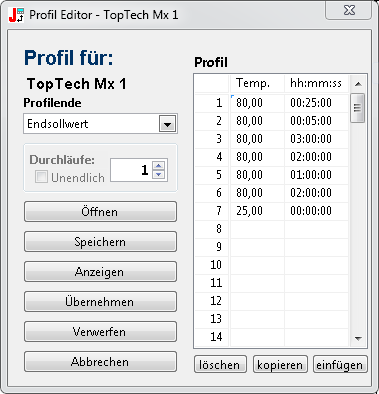
\includegraphics[width=0.5\textwidth]{img/julabo_5}
	\caption{Profileditor in \textsc{Easy Temp}}
	\label{fig:tprofil}
\end{figure}
\FloatBarrier
%Ende

\subsection{Dosierung mit Pumpen}
 


